\documentclass{beamer}

\usepackage[T2A]{fontenc}
\usepackage[utf8]{inputenc}
\usepackage[english,russian]{babel}
\usepackage{amssymb,amsfonts,amsmath,mathtext}
\usepackage{cite,enumerate,float,indentfirst}

\usepackage{graphicx}
\usepackage{booktabs}
\usepackage{tabularx}

\usepackage{qtree}    % regular trees (e.g. GB style)
\usepackage{gb4e}     % numbered lists for linguistic examples

\graphicspath{{images/}}

\usetheme{Rochester}
\usecolortheme{seagull}

\setbeamertemplate{footline}{\scriptsize{\hspace*{0.4cm}\insertframenumber}\vspace*{0.3cm}}
\beamertemplatenavigationsymbolsempty

\errorcontextlines 10000

\begin{document}

\title{\large{\sc Уровневая теория и \\формальное моделирование}}
\author{Константин Соколов}
\institute[]{СПбГПУ}
\date{Санкт-Петербург, 2015} 

\begin{frame}
    \thispagestyle{empty}
    \titlepage
\end{frame}

 
%%%%%%%%%%%%%%%%%%%%%%%%%
% 1. Уровневая теория
%%%%%%%%%%%%%%%%%%%%%%%%%

\begin{frame}{}
\begin{center}
	\textbf{Уровневая теория}
\end{center}
\end{frame}

% уровневая теория, понятие интерфейса 
\begin{frame}{Уровни языка (I)}
\setcounter{framenumber}{1}
\begin{itemize}
    \item уровни языка -- автономные ярусы языковой системы
    	\begin{itemize}
			\item лексикон
			\item фонология
			\item морфология
			\item синтаксис
			\item семантика    	
    	\end{itemize}
	\item предпосылка выделения уровней -- формальное моделирование (определение единиц уровня, критериев их разграничения)    	
\end{itemize}
\end{frame}

\begin{frame}{Уровни языка (II)}
\begin{itemize}
	\item уровни оперируют однородными единицами
	\item единицы одного уровня способны вступать в синтагматические и парадигматические отношения (слова -- словосочетания)
	\item единицы разных уровней способны вступать в иерархические отношения (фонемы -- морфемы -- словоформы)
	\item эмические (фонемы, морфемы) и этические (фоны, морфы) единицы 
\end{itemize}
\end{frame}

\begin{frame}{Уровни языка (III)}
\begin{itemize}
	\item интерфейсы 
	    \begin{itemize}
	    	\item фонолого-морфологический
	    	\item морфолого-синтаксический
	    	\item синтактико-семантический
	    \end{itemize}
	\item интерфейсы в минимализме 
		\begin{itemize}
			\item артикуляторно-перцептивный (фонологический)
			\item интенционально-концептальный (семантический)
		\end{itemize}
\end{itemize}
\end{frame}


%%%%%%%%%%%%%%%%%%%%%%%%%%%%%%%%%
% 2. Формальное моделирование
%%%%%%%%%%%%%%%%%%%%%%%%%%%%%%%%%

\begin{frame}{}
\begin{center}
	\textbf{Формальное моделирование}
\end{center}
\end{frame}

% Примеры для начала обсуждения
\begin{frame}{Вопросы для начала обсуждения}
\begin{itemize}
	\item какой смысл нужно вкладывать в утверждение, что формализм адекватен естественному языку (корректно отражает)?
	\item как следует понимать известное утверждение, что естественный язык не является контекстно-свободным?
	\item каково соотношение между формальной моделью и используемым ею формализмом?
\end{itemize}
\end{frame}

% Сравнение формальной грамматики естественного языка и языка программирования. Во втором случае грамматика носит нормативный характер, в первом – характер формальной модели.
\begin{frame}{Естественный язык vs. язык программирования}
\begin{itemize}
	\item грамматика языка программирования -- нормативная
	\item формальная грамматика естественного языка -- модель
\end{itemize}
\end{frame}

\begin{frame}{Требования к формальной модели}
\begin{itemize}
	\item сознательное ограничение ``зоны ответственности'' (не должна объяснять всё)
	\item не противоречит фактам (наблюдениям)
	\item позволяет делать предсказания, подтверждаемые экспериментом
	\item не делает предсказаний, противоречащих известным данным
\end{itemize}
\bigskip
Следствие: возможность сосуществования разных теорий\\ (ср. лагранжев и гамильтонов формализм в механике).
\end{frame}

% Примеры лингвистических теорий
\begin{frame}{``Большие'' лингвистические теории}
\begin{itemize}
	\item стандартная модель
	\item теория управления и связывания (GB)
	\item минимализм
	\item вершинная грамматика составляющих (HPSG)
	\item лексико-функциональная грамматика (LFG)
	\item модель <<смысл $\leftrightarrow$ текст>> (МСТ) -- \textit{с оговорками}
\end{itemize}
\end{frame}

\begin{frame}{Частные лингвистические теории (I)}
\begin{itemize}
	\item генеративная фонология (SPE, 1968)
	\item автосегментная фонология
	\item распределенная морфология
	\item теория оптимальности
	\item просодическая морфология
\end{itemize}
\end{frame}

\begin{frame}{Частные лингвистические теории (II)}
\begin{itemize}
	\item универсальная грамматика Р.~Монтегю
	\item генеративный лексикон Дж.~Пустейовского
	\item lingua mentalis А.~Вежбицкой
	\item лексическая семантика на основе семантической деривации (Е.~В.~Падучева 2004)
	\item теоретико-типовая лексическая семантика (Sandu 1994, Asher 2010)
\end{itemize}
\end{frame}

\begin{frame}{Общая характеристика}
Динамические модели:\\
\medskip
\begin{itemize}
	\item порождающие, производящие, объяснительные
	\item мыслятся как ``функционирующий механизм''
	\item противопоставляются описательным теориям
\end{itemize}
\medskip
{\small Термин \textit{динамические модели} встречается, напр., в книгах С.~В.~Кодзасов, О.~Ф.~Кривнова ``Общая фонетика'', Е.~В.~Падучева ``Динамические модели в семантике лексики''.}
\end{frame}

\begin{frame}{Примеры формализмов (I)}
\begin{itemize}
	\item грамматики непосредственных составляющих\\(phrase structure grammars)
	\item грамматики зависимостей (dependency grammars)
	\item грамматики, задающие слабо контекстно-зависимые языки (TAG и др.)
	\item контекстно-свободные грамматики (CFG)
	\item категориальные грамматики (AB-грамматики, исчисление Ламбека, комбинаторные категориальные грамматики, Type-Logical Grammar)
\end{itemize}
\end{frame}

\begin{frame}{Примеры формализмов (II)}
\begin{itemize}
	\item унификационные грамматики
	\item окрестностные грамматики
	\item теория типов ($\lambda_\to$ в формальной семантике, Мартин-Лёф в лексической семантике)
	\item универсальная алгебра (синтактико-семантический интерфейс в грамматике Монтегю)
	\item соответствие Карри-Ховарда (синтактико-семантический интерфейс в TLG)
\end{itemize}
\end{frame}

\begin{frame}{}
\begin{center}
	\textbf{Пример лингвистической теории: $X'$-теория}
\end{center}
\end{frame}

\begin{frame}{Факт существования частей речи}
Различные морфологические и синтаксические свойства:\\
\medskip
\begin{exe}
	\ex различные парадигмы словоизменения
	    \begin{xlist}
		    \ex[]{дом, дома, дому, дом, домом, доме}
            \ex[]{иду, идёшь, идёт}
            \ex[]{понимай} 
        \end{xlist}
    \ex различная дистрибуция
	    \begin{xlist}
		    \ex[]{to drink water}
            \ex[]{to water the flowers}
        \end{xlist}
\end{exe}
\end{frame}

\begin{frame}{Факт существования синтаксических групп (I)}
Допустимость топикализации:\\
\medskip
\begin{exe}
	\ex глагольная группа
	    \begin{xlist}
            \ex[]{Он не способен \textit{совершить такую подлость}.}
		    \ex[]{\textit{Совершить такую подлость} он не способен.}
        \end{xlist}
	\ex именная группа
	    \begin{xlist}
            \ex[]{Я очень давно не видел \textit{Ивана}.}
		    \ex[]{\textit{Ивана} я очень давно не видел.}
        \end{xlist}
	\ex предложная группа
	    \begin{xlist}
            \ex[]{Нельзя ничего класть \textit{на этот стол}.}
		    \ex[]{\textit{На этот стол} нельзя ничего класть.}
        \end{xlist}
\end{exe}
\end{frame}

\begin{frame}{Факт существования синтаксических групп (II)}
Возможность замещения местоимением:\\
\medskip
\begin{exe}
    \ex 
	    \begin{xlist}
		    \ex[]{Что вы скажете об \textit{этом человеке, который предлагал нашей фирме очень выгодную операцию с ценными бумагами}?}
            \ex[]{Я скажу, что \textit{он} жулик.}
        \end{xlist}
    \ex[*]{Что вы скажете об этом \textit{нём}, который предлагал нашей \textit{ей} очень выгодную \textit{её} с \textit{ними}?}
\end{exe}
\end{frame}

\begin{frame}{Факт существования внутренней структуры группы}
\begin{exe}
    \ex 
	    \begin{xlist}
		    \ex[]{What are you going to do?}
            \ex[]{Help you.}
        \end{xlist}
	\ex {\small вершину группы нельзя удалить}
	    \begin{xlist}
		    \ex[]{I am trying to \textit{help you}.}
            \ex[]{I am trying to \textit{help}.}
            \ex[*]{I am trying to \textit{you}.}
        \end{xlist}
	\ex {\small нельзя заменить группой другого класса (NP на VP)}
	    \begin{xlist}
		    \ex[]{\textit{You} are difficult.}
            \ex[]{\textit{Help you} are difficult.}
        \end{xlist}
\end{exe}
\end{frame}

\begin{frame}{Факт единообразия структуры групп различных классов}
Сходные механизмы расширения групп:\\
\medskip
\begin{itemize}
    \item[NP:]{дом, большой дом, дом мельника, большой дом мельника, большой и красивый дом старого мельника}
    \item[VP:]{прятался, прятался в траве, часто прятался, часто прятался в зелёной траве}
    \item[AP:]{довольный, довольный собой, очень довольный собой, очень довольный собой и успехами своих детей}
    \item[PP:]{после дождя, после дождя в четверг, вскоре после холодного осеннего дождя, вскоре после непродолжительного дождя в четверг}
\end{itemize}
\end{frame}

\begin{frame}{Вывод}
\begin{quote}
``Предложение не составляется непосредственно из слов как из конститутивных элементов и не разложимо непосредственно на слова.''
\end{quote}
\begin{flushright}
\textit{{\small Золотова (1981), цит. по Тестелец (2001), стр. 144}}
\end{flushright}
\end{frame}

\begin{frame}[fragile]{$X'$-теория (базовая структура)}
Существует базовая структура группы:\\
\bigskip
\Tree [.XP [.Spec ] [.X' [.Adjunct ] [.X' [.X^0 ] [.Complement ] ] ] ]\\
\bigskip
Терминология: спецификатор, адъюнкт, вершина $X^0$, комплемент, первая проекция вершины $X'$, вторая (максимальная) проекция вершины $X'' = XP$, фразовая категория (``класс группы'')
\end{frame}

\begin{frame}[fragile]{$X'$-теория (вершина и комплемент)}
\begin{center}
\Tree [.NP [.N^0 портрет ] \qroof{короля Испании}.NP ]
\Tree [.VP [.V^0 бежать ] \qroof{на крышу}.PP ]\\
\medskip
\Tree [.PP [.P^0 после ] \qroof{выступления}.NP ]
\Tree [.AP [.A^0 сердитый ] \qroof{на весь мир}.NP ]
\end{center}
\end{frame}

\begin{frame}[fragile]{$X'$-теория (спецификатор и адъюнкт)}
\begin{center}
\Tree [.NP [.Spec мой ] [.N' [.N^0 дом ] ] ]
\Tree [.PP [.Spec сразу ] [.P' [.P^0 после ] \qroof{дождя}.NP ] ]
\Tree [.AP [.Spec очень ] [.A' [.A^0 сердитый ] \qroof{на весь мир}.PP ] ]
\end{center}
\end{frame}

\begin{frame}[fragile]{$X'$-теория (параметр расположения вершины)}
\begin{center}
\Tree [.XP [.Spec ] [.X' [.X^0 ] [.Compl ] ] ]
\Tree [.XP [.Spec ] [.X' [.Compl ] [.X^0 ] ] ]
\end{center}
\medskip
\begin{exe}
	\ex 
		\gll teburu-no ue-ni aru hon-o kure!\\
             стол.GEN на.LOC находящийся книга.ACC дай\\
		\glt \textit{дай книгу, которая лежит на столе!}
\end{exe}	
\end{frame}

\begin{frame}[fragile]{$X'$-теория (объяснительная сила)}
\begin{itemize}
	\item любая группа обладает вершиной, грамматические свойства вершины определяют свойства всей группы (принцип эндоцентричности)
	\item любой элемент синтаксической структуры является либо вершиной группы, либо проекцией вершины
	\item параметр расположения вершины позволяет объяснить явления правого и левого ветвления
\end{itemize}
\end{frame}



\begin{frame}{}
\begin{center}
	\textbf{Споры}
\end{center}
\end{frame}

\begin{frame}{Мельчук и Тестелец о микроскопе}
\begin{center}
        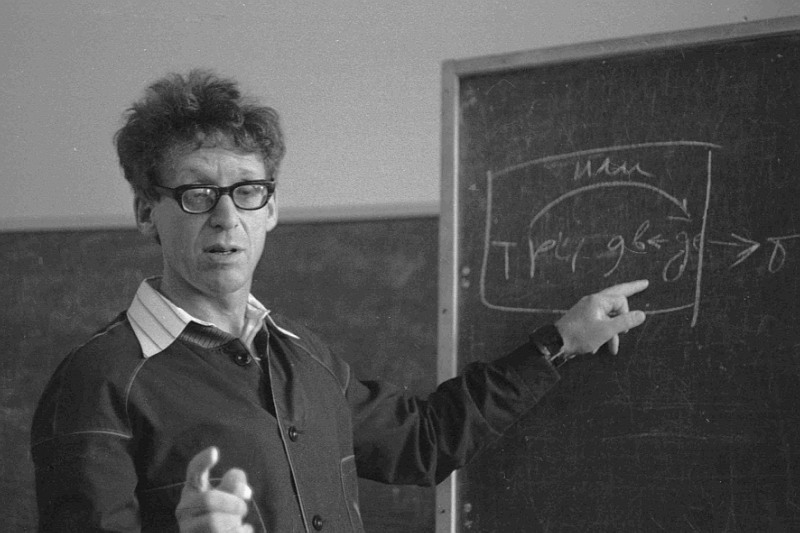
\includegraphics[width=0.506\textwidth]{melcuk.jpg}
        \hfill
        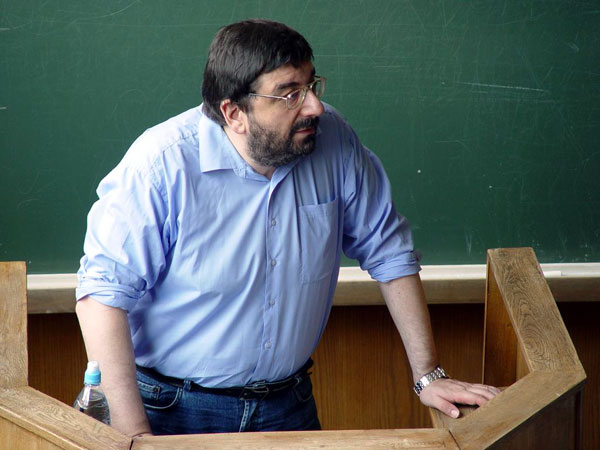
\includegraphics[width=0.45\textwidth]{testelets.jpg}
\end{center}
\end{frame}

\begin{frame}{Мельчук и Тестелец о микроскопе}
\ \\
{\small <<Функциональная модель X предмета или явления Y -- это искусственно созданная система, быть может, совершенно иной физической природы, нежели Y, но такая, что если её поместить в обстановку, в которой действует Y, то она будет вести себя -- во всяком случае, в интересующем нас аспекте! -- достаточно похоже на Y, а в идеале -- неотличимо от Y. \dots [В]нутреннее, структурное тождество X-а и Y-а всё равно не гарантировано. [\dots] ``Создание модели есть доказательство ясности понимания.'' (Miller, Gallanter, Pribram 1960)>> \textit{(И.~А.~Мельчук, МСТ, с. 11-12)}}\\
\end{frame}

\begin{frame}{Хомский и Норвиг о статистических моделях}
\begin{center}
        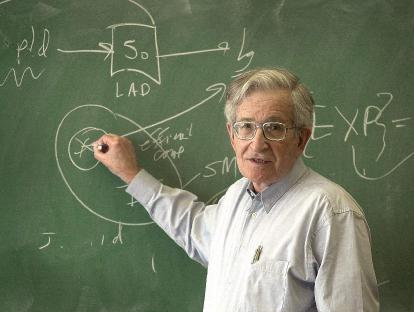
\includegraphics[width=0.41\textwidth]{chomsky.jpg}
        \hfill
        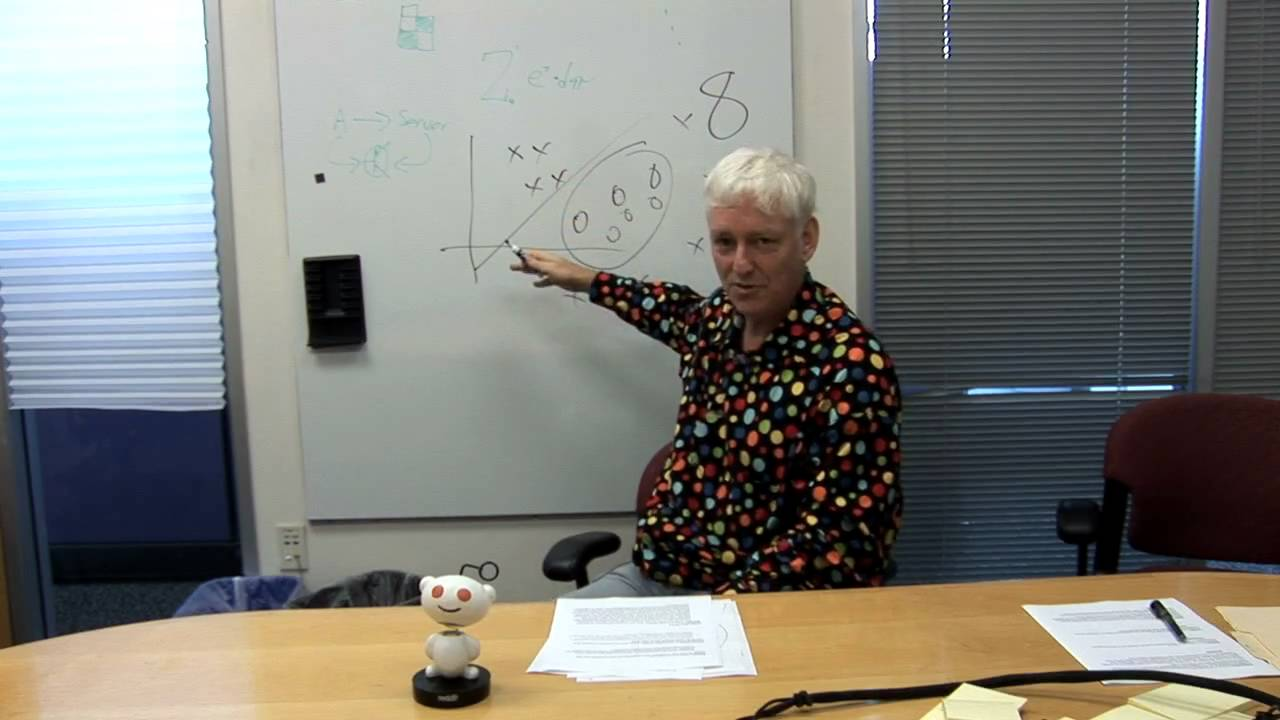
\includegraphics[width=0.55\textwidth]{norvig.jpg}
\end{center}
Домашнее задание: \texttt{http://norvig.com/chomsky.html}
\end{frame}


%%%%%%%%%%%%%%%%%%%%%
%   3. Обзор курса
%%%%%%%%%%%%%%%%%%%%%     

\begin{frame}{}
\begin{center}
	\textbf{Обзор курса}
\end{center}
\end{frame}

\begin{frame}{Основы}
\begin{itemize}
	\item уровневая теория и формальное моделирование
	\item языковое разнообразие, письменность и нормализация текста
	\item неоднозначность
\end{itemize}
\end{frame}

\begin{frame}{Морфология}
\begin{itemize}
	\item морфология и лексикон, лексикализм vs. распределенная морфология, разграничение морфологического и синтаксического уровней
	\item морфология и грамматическая семантика, грамматические признаки, корпуса с морфологической разметкой
\end{itemize}
\end{frame}

\begin{frame}{Синтаксис}
\begin{itemize}
	\item формальный синтаксис, mild context sensitivity и ``тезис Джоши'', результат о слабой эквивалентности TAG, LIG, HG и CCG
	\item синтаксический разбор как логический вывод, алгоритм Кока-Янгера-Касами для TAG
	\item задача контроля выразительности синтаксического формализма (унификационные  грамматики и MMCCG)
	\item корпуса с синтаксической разметкой, обучение грамматики по корпусу (PCFG, LTAG и др.)
\end{itemize}
\end{frame}

\begin{frame}{Семантика}
\begin{itemize}
	\item семантические роли, тета-теория, предикатно-аргументная структура, FrameNet
	\item принцип композициональности и формальная семантика (Монтегю)
	\item синтактико-семантический интерфейс (CFG/FOL, CCG/HLDS, Glue, TLG и соответствие Карри-Ховарда)
	\item дистрибутивная семантика и композициональные дистрибутивные семантические модели
\end{itemize}
\end{frame}

\begin{frame}{Приложения}
\begin{itemize}
	\item извлечение информации
	\item понимание естественного языка
\end{itemize}
\end{frame}


%%%%%%%%%%%%%%%
% 3. Литература к курсу
%%%%%%%%%%%%%%%%

\begin{frame}{}
\begin{center}
	\textbf{Литература к курсу}
\end{center}
\end{frame}

\begin{frame}{По теоретической лингвистике (I)}
\begin{itemize}
	\item В. А. Плунгян. Общая морфология: Введение в проблематику. М.: Эдиториал УРСС, 10, 2000.
	\medskip
	\item В. А. Плунгян. Введение в грамматическую семантику: грамматические значения и грамматические системы языков мира: учебное пособие. РГГУ, 2011.
	\medskip
	\item Я. Г. Тестелец. Введение в общий синтаксис. РГГУ, 2001.
\end{itemize}
\end{frame}

\begin{frame}{По теоретической лингвистике (II)}
\begin{itemize}
	\item Ю. Д. Апресян. Идеи и методы современной структурной лингвистики. (Краткий очерк). 1966.
	\medskip
	\item О. В. Митренина, Е. Е. Романова, Н. А. Слюсарь. Введение в генеративную грамматику. URSS, 2012.
	\medskip
	\item И. М. Кобозева. Общая семантика.
	\medskip
	\item Э. Бах. Неформальные лекции по формальной семантике.
\end{itemize}
\end{frame}


\begin{frame}{По компьютерной лингвистике \\и информационному поиску}
\begin{itemize}
	\item Леонтьева Н. Н. Автоматическое понимание текстов. Системы, модели, ресурсы. 2006.
	\medskip
	\item К. Маннинг, П. Рагхаван и Х. Шютце. Введение в информационный поиск. 2011.
	\medskip
	\item D. Jurafsky, J. Martin. Speech and Language Processing: An Introduction to Natural Language Processing, Computational Linguistics, and Speech Recognition. 2009.
\end{itemize}
\end{frame}

\begin{frame}{По формальным языкам}
\begin{itemize}
	\item Дж. Хопкрофт, Р. Мотвани, Дж. Ульман. Введение в теорию автоматов, языков и вычислений.
	\medskip
	\item А. Ахо, М. Лам, Р. Сети, Дж. Ульман. Компиляторы: принципы, технологии и инструментарий. М., 2008.
	\medskip
	\item L. Kallmeyer. Parsing beyond context-free grammars. Springer Science \& Business Media, 2010.
	\medskip
	\item N. Francez and Sh. Wintner. Unification grammars. Cambridge University Press, 2011.
	\medskip
	\item R. Moot, Ch. Retor\'e. The Logic of Categorial Grammars. Springer-Verlag, 2012.
\end{itemize}
\end{frame}


\begin{frame}{}
\begin{center}
	\textbf{Домашнее задание}
\end{center}
\end{frame}

\begin{frame}{Домашнее задание}
\begin{center}
{\small P. Norvig. On Chomsky and the Two Cultures of Statistical Learning.}\\
\medskip
\texttt{http://norvig.com/chomsky.html}
\end{center}
\end{frame}


\begin{frame}{}
    \thispagestyle{empty}
    \begin{center}
        {\large Спасибо!}
    \end{center}
\end{frame}


\end{document}
